\documentclass[conference]{IEEEtran}
\IEEEoverridecommandlockouts
% The preceding line is only needed to identify funding in the first footnote. If that is unneeded, please comment it out.
\usepackage{cite}
\usepackage{amsmath,amssymb,amsfonts}
\usepackage{algorithmic}
\usepackage{graphicx}
\usepackage{textcomp}
\usepackage{xcolor}
\def\BibTeX{{\rm B\kern-.05em{\sc i\kern-.025em b}\kern-.08em
    T\kern-.1667em\lower.7ex\hbox{E}\kern-.125emX}}
\begin{document}

\title{ADLR WS21 - Final Report Team 04 \\ Harnessing Reinforcement Learning for Neural Motion Planning\\
}

\author{\IEEEauthorblockN{Marc Hauck}
\IEEEauthorblockA{\textit{Robotics, Cognition, Intelligence} \\
\textit{Technical University of Munich}\\
Munich, Germany \\
ge65qoy@mytum.de}
\and
\IEEEauthorblockN{Baris Tura}
\IEEEauthorblockA{\textit{Robotics, Cognition, Intelligence} \\
\textit{Technical University of Munich}\\
Munich, Germany \\
baris.tura@tum.de}}

\maketitle

\begin{abstract}
	In this work, we show how motion planning problems for mobile and planar robots can be solved by using Reinforcement Learning. Starting with a discrete environment and slowly increasing the complexity by using a continuous environment, adding obstacles and constraining the robot's movements to a kinematic, we gradually developed an agent that is able to find a goal in unseen environments with various obstacles. Besides that, we showed that for planar robots, learning the kinematic is a crucial problem that should be addressed separately before performing motion planning tasks.
\end{abstract}

\section{Introduction}
Motion planning is an important discipline in robotics. However, traditional methods might not be able to find paths through narrow passages and often suffer from slow convergence. Using Reinforcement Learning to solve motion planning tasks can solve both of these problems at once, being able to actively explore the environment and to find feasible paths quickly.

 In this work, we aim to harness Reinforcement Learning algorithms to guide a robotic arm with up to three degrees of freedom (DoF) to its goal through an unknown environment, i.e. the instantaneous locations of obstacles are unknown to the agent. To achieve this, we started with a point robot that can freely move in a two-dimensional environment (further referred to as "mobile robot" setting) and gradually increased the complexity of the environment by adding more obstacles. After that, we transferred the obtained results to 2-DoF and 3-DoF planar robot arms and conducted further experiments.

\section{Related Work}

Previous works consist of motion planning in static environments for joint robots, and motion planning in dynamic environments for mobile robots. 

Jurgenson et al. \cite{b1} propose an algorithm based on Deep Deterministic Policy Gradient (DDPG), enriched with expert knowledge for a planar 3-DoF robot in an unknown environment. They claim that supervised learning is heterogeneous in terms of data distribution and lacks sufficient data close to object boundaries; and that imitation learning leaves no room for exploration, especially in unseen environments as the expert never collides with the objects. Their results obtained with the expert knowledge supported algorithm named DDPG-MP show superior results to those of classic approaches using DDPG and Hindsight Experience Replay (HER).

Prokudin et al. \cite{b2} present a framework that simplifies and speeds up point cloud processing. To do so, 3D point clouds are projected onto a Basis Point Set (BPS). This BPS consists of a fixed set of so-called basis points that are sampled throughout the environment. Projection of all points onto the BPS yields a distance vector, each entry of the vector representing the distance of the corresponding basis point to the closest point in the cloud, or the closest obstacle respectively. This approach eliminates the issue of varying input shapes as the BPS is predetermined and the resulting vector is always of the same length. It also helps alleviate the problem of possible permutations as each basis point has a fixed corresponding entry in the distance vector. As point clouds are often used as obstacle representation for 3D motion planning tasks, this approach can also be converted to the 2D case, offering an alternative obstacle representation.

Wang et al. \cite{b3} guide an agent through a 2D environment comprising of static and dynamic obstacles using convolutional neural networks for scene understanding and an LSTM+MLP network for action selection. Here, they make use of A*-search as global guidance to enforce minimal traversal through the environment while still avoiding the dynamic obstacles. All the obstacles are unknown a priori and are perceived within a certain field of view by the robot. For action selection, classic DDQN algorithm is used in conjunction with an LSTM network to have temporal reasoning. They name the approach Globally Guided Reinforcement Learning and obtain state-of-the-art results. 

\section{Experiments}

\subsection{Methods}

\subsubsection{Environment Representation}

There are three possibilities for representing the environment and specifically the obstacles. The first one is a purely positional representation, where for each obstacle the corresponding $x-$ and $y-$coordinates are embedded, which leads to a matrix of size $n_{obstacles} \times 2$ as the observation space. This approach is simple and quite easy to compute. Nonetheless, it is also very limited as it lacks expressiveness and does not allow to alter with the number of obstacles in runtime. 
The second option is making use of raw images. Here, at each timestep the environment is rendered, and the resulting RGB tensor is employed as the observation space of the network. This approach is highly expressive. Everything that the agent may need is readily available to it and the agent can have immediate feedback concerning its actions. However, this method leads to a large state space and an accordingly large network. To put in perspective, a square RGB image of size 400 pixels put into use in a DDPG algorithm with 1 million buffer size and 128 batch size requires 437 GB of memory. Making updates to such a big network is cumbersome. 

\begin{figure}[!t]
	\centering
	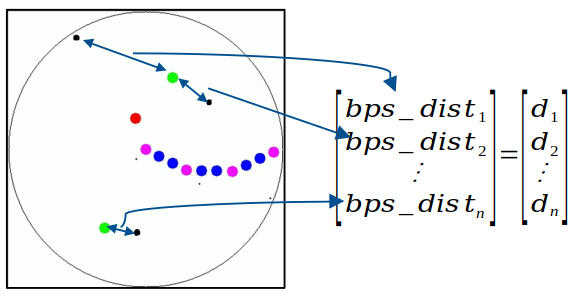
\includegraphics[width=2.5in]{bpsill}
	\caption{Basis Points Set as Environment Representation. The resulting vector stays the same, regardless of obstacle number, position or shape.}
	\label{fig1}
\end{figure}

The last option is to use Basis Points Sets, as mentioned in section II and illustrated in Figure \ref{fig1}. This option finds a balance between the other two in terms of expressiveness and simplicity. It is still a relatively expressive method, though not as much as raw images; and it is considerably simple and small in size even though more complex compared to the purely positional representation.

\subsubsection{Runtime Options}

The next set of methods concern the runtime and the way learning is done. The first option is simple vanilla learning, during which the environment is directly presented to the agent at once, the way it is desired to be in the end. In contrast to that, the other option is curriculum learning, where the learning is kicked off with a relaxed and simple version of the problem, and the difficulty is increased as learning progresses. The idea behind curriculum learning is that the agent can carry over what it has learned at each curricular timestep to the next one. Figure \ref{fig2} illustrates the concept of curriculum learning applied on number of obstacles in the environment. Here, the environment starts with two obstacles. Once the agent can perform well on two obstacles, the number of obstacles is increased to 3 and consequentially to 4. After the individual transitions between curricular steps, the agent does not need to learn its kinematic again, but only needs to readjust itself according to the changes made in the environment.

\begin{figure}[!t]
	\centering
	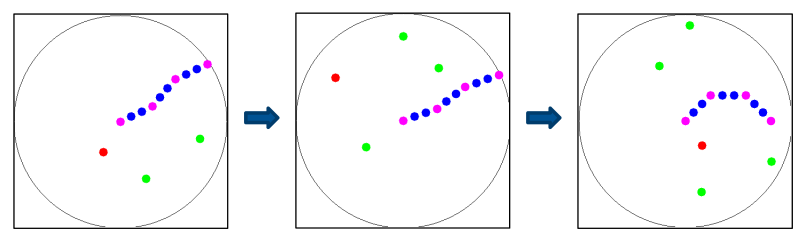
\includegraphics[width=3.2in]{currlearning}
	\caption{Curriculum learning concerning number of obstacles. The number of obstacles is increased at each step.}
	\label{fig2}
\end{figure}

\subsection{Mobile Robot}

In all our experiments, we used the Stable-Baselines 3 (SB3) library and an environment inherited from the Open AI gym class, together with the reinforcement learning algorithm Proximal Policy Optimization (PPO), as was suggested by the SB3 documentation for problems similar to ours. 

We first performed motion planning for an agent in an empty 10 x 10 grid world environment with no obstacles, fixed start and goal positions and a sparse reward of 1 for finding the goal and 0 else. Using a discrete observation and action space, the experiments needed only little computation time and the agent was able to overfit to this environment quickly.

In a second step, we added obstacles to the environment and initially rewarded a collision with -1. Adding the obstacles that were initially represented by their positions led to a massive increase in computation time as with the number of obstacles the dimension of the observation space was increased proportionally. Additionally, it required the introduction of weights for the positive and negative rewards, so that the agent did not overfit on either ignoring the obstacles or not trying to get to the goal at all to not get a negative reward. After increasing the number of training steps and finding suitable reward weights by using binary search, we were able to successfully train the agent in this environment.

\begin{figure}[htbp]
	\centerline{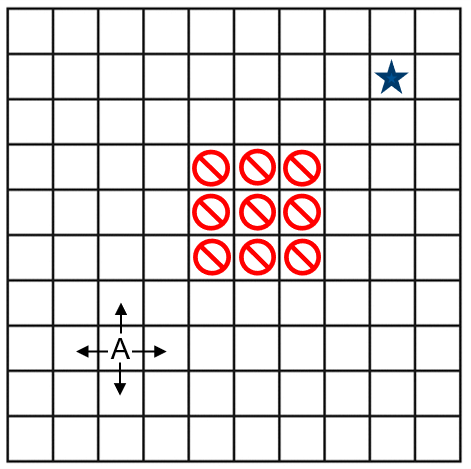
\includegraphics{discrete.png}}
	\caption{10x10 discrete environment: The agent (A) has to find the goal (star) without colliding with the obstacles (do-not-cross signs).}
	\label{fig3}
\end{figure}

Next, we transformed the environment to a continuous one that was normalized to [-1, 1] x [-1, 1]. To enable the agent to freely move in the continuous space, the two-dimensional action space was initially set to [-1, 1] for the agent's velocity in x- and y-direction. Later, this action space was only used to determine the direction of the agent's velocity vector in order to guarantee a fixed step size. This led to a drastic reduction of action space and required training time. 

As the rewards from the discrete environment proved to be too sparse in the continuous environment, we had to change the reward function in a way that guided the agent more towards the goal. To do that, we rewarded the negative distance of the agent to the goal in every step. This led to good results in empty environments with little training time.

Similar to the discrete environment, we then added obstacles and provided a negative reward for a collision. We were able to successfully guide the agent to the goal for up to three obstacles, observing an increase of required training time with an increasing number of obstacles again. For environments with more obstacles, the agent was not able to find the goal reliably anymore, even with the training time being one order of magnitude higher than before.

This problem is caused by the varying size and permutation of the observation space: With each additional obstacle, the dimension of the observation space increases by two, adding another x- and y-position. Furthermore, possible permutations of the observation space prevent the agent from gaining a solid understanding of its environment. To cope with these problems, we adopted the idea of Basis Point Sets \cite{b2} for our two-dimensional case, which led to significantly better results. Finally, we tried to even improve them by parameter tuning. The results of these experiments are discussed in section IV.

\subsection{Planar Robot Arms}

In the second part of our work, we focused on motion planning for planar robot arms. While still using a 2D environment, the constraints of the robot kinematics increased the complexity of this task. Although only performing experiments with 2- and 3-DoF robots, we implemented a kinematic that is scalable for arbitrary DoF and shown in Figure \ref{fig4}: The robot's workspace is the unit circle, setting the total arm length to 1. As the link lengths should all be the same, they resulted from the number of DoF. To make collision checking easy for the whole robot arm, the joints as well as the end effector and the links are represented as circles, with multiple circles being used for each link so obstacles could not fit in the gap between two circles. 

\begin{figure}[htbp]
	\centerline{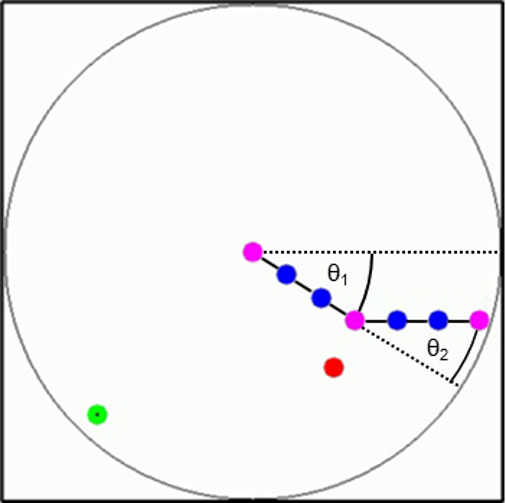
\includegraphics{2dof.png}}
	\caption{Environment for a 2-DoF planar robot. The two joints with joint angles $\theta_1$ and $\theta_2$ as well as the end effector are represented by pink circles, while the links are represented by blue circles.}
	\label{fig4}
\end{figure}

Although the task space was still continuous, the action space of the robot changed to discrete. In every step, each drive can rotate $\pm 1^{\circ}$. While collisions with obstacles are checked for all robot parts, the goal has to be reached with the robot's end effector for a run to be successful. 

Similar to the mobile robot setting, the robot first had to find the goal in an empty environment. This simple problem already proved to be much more difficult for the planar robot compared to the mobile robot. The reason for that is that the robot does not know its kinematic, the mapping from joint space to task space and vice versa. Therefore, the reward function that before guided the mobile robot to the goal in cartesian space had to be adapted. As the planar robot takes actions in joint space, it is more convenient to also guide the robot towards the goal in joint space. Therefore, the goal had to be sampled in joint coordinates instead of cartesian coordinates. 

After the robot was able to find the goal in an empty environment, more obstacles were introduced step by step. For more than one obstacle, we constrained the obstacle sampling such that the first joint could still move freely, ensuring that it was still possible for the robot to reach the goal in most cases. Nevertheless, the introduction of obstacles complicated the task because of the robot's kinematic again as the obstacles are sampled in task space. In contrast to the goal which is often available in joint coordinates in real-world problems, it is not realistic to sample the positions of obstacles in joint space. To gain an understanding of when collisions happen and which action caused them, the agent therefore has to learn its kinematic in addition to the environment representation. This is the reason why the planar robots were a lot harder to train than the mobile robots.

\section{Results}

\subsection{Mobile Robot}

\begin{figure}[htbp]
	\centerline{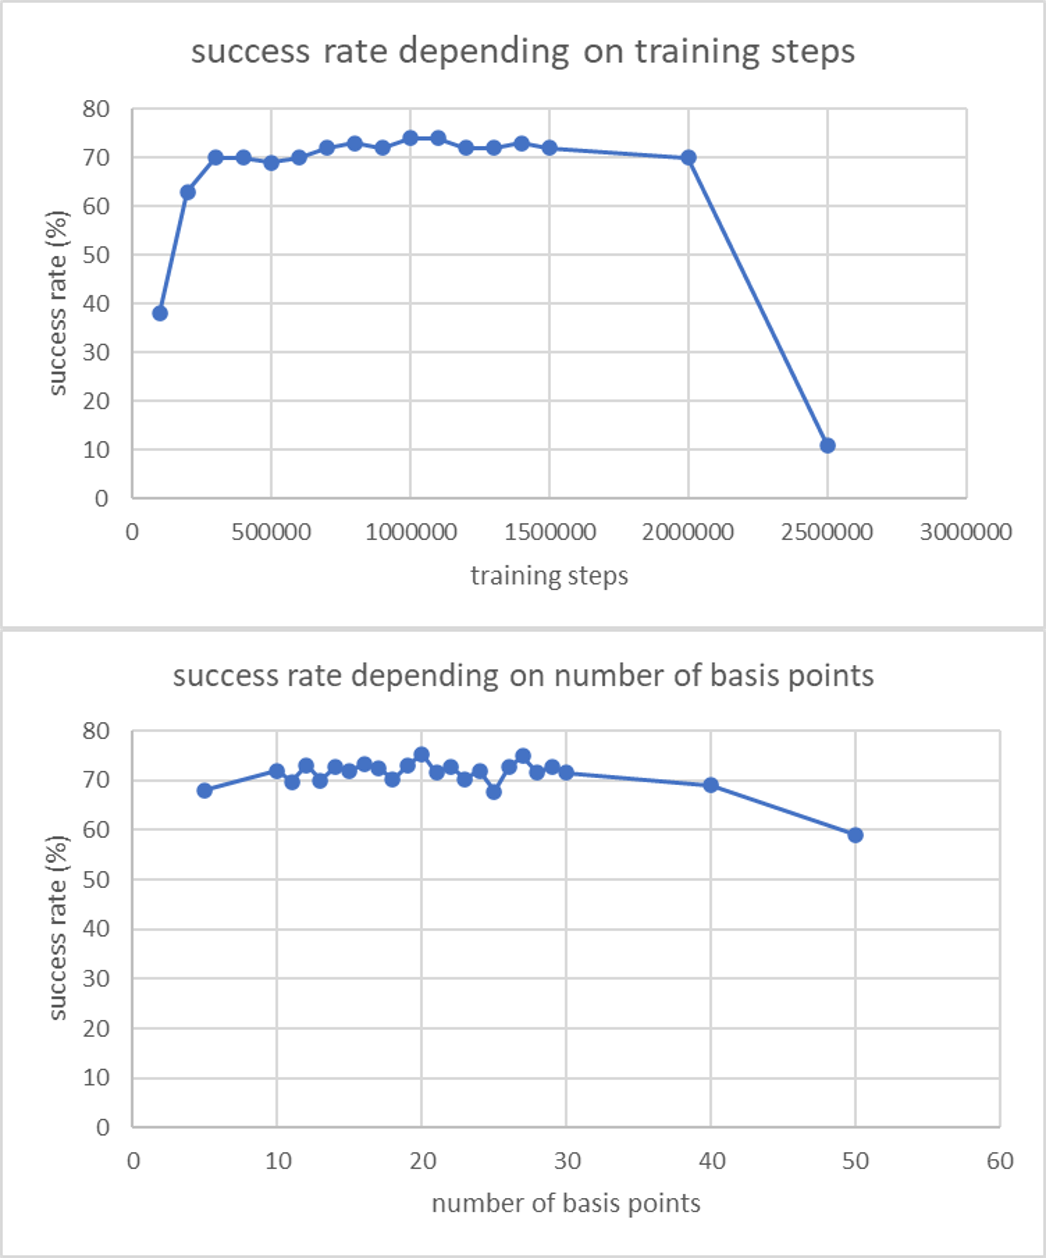
\includegraphics{mobile.png}}
	\caption{Even for optimized number of training steps and basis points, the success rate does not exceed 80\%. Further increasing them leads to a performance breakdown.}
	\label{fig5}
\end{figure}

For the mobile robot, we tried to optimize the success rate of the agent in an environment with ten randomly sampled obstacles. We first tried to find good initial parameters and always achieved a success rate of 70 to 80\%. To improve these numbers, we iteratively optimized the number of training steps and the number of basis points. As shown in Figure \ref{fig5}, neither the optimal number of training steps nor the optimal number of basis points led to an improvement. Interestingly, further increasing the number of training steps and basis points also could not improve the agent's performance. This most likely happens because of overfitting or exploding and vanishing gradients in the underlying neural network. This problem could be tackled by tuning the network's hyperparameters which lies beyond the scope of this work.

\subsection{2 DoF Planar Robot Arm}

In Table \ref{table:1}, we present the success rate in percentage over a 1000 validation runs for the 2-DoF planar robot. Here, a run is called successful if the agent finds the goal without colliding with any obstacles. The algorithm that was used for these experiments is again PPO. We also experimented DDPG and Soft Actor Critic (SAC) as well, yet although these two algorithms show good results very quickly, PPO leads to better results in the long run. As mentioned earlier, the difficult part of this problem is not the complexity of the environment but rather learning the robot's kinematic. As such, we draw attention to comparison cases where the environment elements are kept fixed, that is, different combinations of options for a given number of obstacles. 
For the first case with one obstacle, it is seen that curriculum learning outperforms vanilla learning, with positional representation having a slight edge over BPS, which is to be expected as the usage of more complex object representation does not lead to better performance for such a simple setting. However, it can also be seen that even for this simple setting the image representation struggles, which gives a hint as to how detrimental large networks can be. 
For the second and third case with two and seven obstacles respectively, we see that the combination of curriculum learning and BPS outperforms all other combinations, with 70\% and 29\% success rate respectively. Based on the reasonings given above, such a result could be expected. Even though this is only a small set of experiments, we can claim that for the 2-DoF case, the combination of curriculum learning and BPS is the choice to be made. 

\begin{table}[!t]
	\renewcommand{\arraystretch}{1.3}
	\caption{Results for 2-DoF Planar Robot}
	\label{table:1}
	\centering
	\begin{tabular}{c|ccc|ccc|}
		\cline{2-7}
		& \multicolumn{3}{c|}{Vanilla}                                       & \multicolumn{3}{c|}{Curriculum}                                    \\ \cline{2-7} 
		& \multicolumn{1}{c|}{Positional} & \multicolumn{1}{c|}{BPS} & Image & \multicolumn{1}{c|}{Positional} & \multicolumn{1}{c|}{BPS} & Image \\ \hline
		\multicolumn{1}{|c|}{1 Obstacle}  & \multicolumn{1}{c|}{\textbf{84}}          & \multicolumn{1}{c|}{79}   & 70     & \multicolumn{1}{c|}{\textbf{84}}          & \multicolumn{1}{c|}{83}   & 68     \\ \hline
		\multicolumn{1}{|c|}{2 Obstacles} & \multicolumn{1}{c|}{64}          & \multicolumn{1}{c|}{68}   & 51     & \multicolumn{1}{c|}{67}          & \multicolumn{1}{c|}{\textbf{70}}   & 54     \\ \hline
		\multicolumn{1}{|c|}{3 Obstacles} & \multicolumn{1}{c|}{27}          & \multicolumn{1}{c|}{28}   & 12     & \multicolumn{1}{c|}{27}          & \multicolumn{1}{c|}{\textbf{29}}   & 13     \\ \hline
	\end{tabular}
\end{table}

\subsection{3 DoF Planar Robot Arm}

\begin{table}[!t]
	\renewcommand{\arraystretch}{1.3}
	\caption{Results for 3-DoF Planar Robot}
	\label{table:2}
	\centering
	\begin{tabular}{c|ccc|ccc|}
		\cline{2-7}
		& \multicolumn{3}{c|}{Vanilla}                                       & \multicolumn{3}{c|}{Curriculum}                                    \\ \cline{2-7} 
		& \multicolumn{1}{c|}{Positional} & \multicolumn{1}{c|}{BPS} & Image & \multicolumn{1}{c|}{Positional} & \multicolumn{1}{c|}{BPS} & Image \\ \hline
		\multicolumn{1}{|c|}{1 Obstacle}  & \multicolumn{1}{c|}{42}          & \multicolumn{1}{c|}{47}   & 39     & \multicolumn{1}{c|}{44}          & \multicolumn{1}{c|}{\textbf{48}}   & 36     \\ \hline
		\multicolumn{1}{|c|}{2 Obstacles} & \multicolumn{1}{c|}{30}          & \multicolumn{1}{c|}{35}   & 35     & \multicolumn{1}{c|}{32}          & \multicolumn{1}{c|}{32}   & \textbf{51}     \\ \hline
		\multicolumn{1}{|c|}{3 Obstacles} & \multicolumn{1}{c|}{7}          & \multicolumn{1}{c|}{\textbf{13}}   & 10     & \multicolumn{1}{c|}{10}          & \multicolumn{1}{c|}{9}   & 11     \\ \hline
	\end{tabular}
\end{table} 

Table \ref{table:2} shows the success rate in percentage over a 1000 validation runs for the 3-DoF planar robot. The setting of the algorithms is similar to the 2-DoF case. 
Looking at the results, a lack of trend is immediately clear. It should be kept in mind that 3-DoF is much more complicated in comparison to 2-DoF in the planar case. For the inverse kinematic problem in the 2 DoF setting, there exist two possible solutions for a given point. In contrast to that, in the 3-DoF setting, there exist infinitely many solutions, and the agent needs to learn to discern between these many solutions. 
For one obstacle, BPS and curriculum learning perform the best. Once the number of obstacles is increased to two, suddenly image representation works better and what is more surprising, for 7 obstacles vanilla learning outperforms curriculum learning. What is happening here is that the agent cannot learn what is at the core of the task, i.e. its kinematic. When this is the case, it does not help any further to employ advanced techniques such as curriculum learning or basis points sets. Thus, we can conclude that for neural motion planning, the robots kinematic should be learned first, and further experiments should follow that.

\section{Conclusion} 

We have shown that for the neural motion planning of a planar robot arm, the main difficulty is not the complexity of the environment but rather learning the inverse kinematics. Through our experiments we have come to the following conclusions:
 \begin{itemize}
\item DDPG and SAC show good results very quickly, but PPO proves to be better in the long run.
\item Basis Points Sets provide a good and balanced solution for environment representation.
\item Curriculum learning highly enhances the results, as long as the fundamentals can be learned.
\end{itemize}
We believe the main and immediate focus of future work should be on learning the robots kinematic, which can be accomplished by means of supplementing measures such as HER or expert knowledge in the form of classical path planning. Once that is accomplished, one can move forward and increase the complexity of the environment by increasing the degrees of freedom, making the obstacles dynamic, or transitioning into a 3D environment.

\begin{thebibliography}{00}
\bibitem{b1} T. Jurgenson and A. Tamar, ``Harnessing reinforcement learning for neural
motion planning'',  \textit{arXiv preprint arXiv:1906.00214}, 2019.
\bibitem{b2} S. Prokudin, C. Lassner, and J. Romero. "Efficient learning on point clouds with Basis Point sets". \textit{Proceedings of the IEEE/CVF International Conference on Computer Vision (ICCV)}, pp. 4332–4341, 2019.
\bibitem{b3} B. Wang, Z. Liu, Q. Li, and A. Prorok, "Mobile robot path planning in dynamic environments through globally guided reinforcement learning",  IEEE Robotics and Automation Letters, 5(4), pp. 6932-6939, 2020.
\end{thebibliography}

\end{document}
